% Options for packages loaded elsewhere
\PassOptionsToPackage{unicode}{hyperref}
\PassOptionsToPackage{hyphens}{url}
%
\documentclass[
  12pt,
]{article}
\usepackage{lmodern}
\usepackage{amssymb,amsmath}
\usepackage{ifxetex,ifluatex}
\ifnum 0\ifxetex 1\fi\ifluatex 1\fi=0 % if pdftex
  \usepackage[T1]{fontenc}
  \usepackage[utf8]{inputenc}
  \usepackage{textcomp} % provide euro and other symbols
\else % if luatex or xetex
  \usepackage{unicode-math}
  \defaultfontfeatures{Scale=MatchLowercase}
  \defaultfontfeatures[\rmfamily]{Ligatures=TeX,Scale=1}
  \setmainfont[]{Times New Roman}
  \setsansfont[]{Quicksand}
\fi
% Use upquote if available, for straight quotes in verbatim environments
\IfFileExists{upquote.sty}{\usepackage{upquote}}{}
\IfFileExists{microtype.sty}{% use microtype if available
  \usepackage[]{microtype}
  \UseMicrotypeSet[protrusion]{basicmath} % disable protrusion for tt fonts
}{}
\makeatletter
\@ifundefined{KOMAClassName}{% if non-KOMA class
  \IfFileExists{parskip.sty}{%
    \usepackage{parskip}
  }{% else
    \setlength{\parindent}{0pt}
    \setlength{\parskip}{6pt plus 2pt minus 1pt}}
}{% if KOMA class
  \KOMAoptions{parskip=half}}
\makeatother
\usepackage{xcolor}
\IfFileExists{xurl.sty}{\usepackage{xurl}}{} % add URL line breaks if available
\IfFileExists{bookmark.sty}{\usepackage{bookmark}}{\usepackage{hyperref}}
\hypersetup{
  pdftitle={Loglinear models and latent class analysis},
  pdfauthor={Pamela Inostroza Fernández},
  hidelinks,
  pdfcreator={LaTeX via pandoc}}
\urlstyle{same} % disable monospaced font for URLs
\usepackage[margin=1in]{geometry}
\usepackage{longtable,booktabs}
% Correct order of tables after \paragraph or \subparagraph
\usepackage{etoolbox}
\makeatletter
\patchcmd\longtable{\par}{\if@noskipsec\mbox{}\fi\par}{}{}
\makeatother
% Allow footnotes in longtable head/foot
\IfFileExists{footnotehyper.sty}{\usepackage{footnotehyper}}{\usepackage{footnote}}
\makesavenoteenv{longtable}
\usepackage{graphicx,grffile}
\makeatletter
\def\maxwidth{\ifdim\Gin@nat@width>\linewidth\linewidth\else\Gin@nat@width\fi}
\def\maxheight{\ifdim\Gin@nat@height>\textheight\textheight\else\Gin@nat@height\fi}
\makeatother
% Scale images if necessary, so that they will not overflow the page
% margins by default, and it is still possible to overwrite the defaults
% using explicit options in \includegraphics[width, height, ...]{}
\setkeys{Gin}{width=\maxwidth,height=\maxheight,keepaspectratio}
% Set default figure placement to htbp
\makeatletter
\def\fps@figure{htbp}
\makeatother
\setlength{\emergencystretch}{3em} % prevent overfull lines
\providecommand{\tightlist}{%
  \setlength{\itemsep}{0pt}\setlength{\parskip}{0pt}}
\setcounter{secnumdepth}{5}
\usepackage[font=small,format=plain,labelfont=bf,up,textfont=normal,up,justification=justified,singlelinecheck=false]{caption} \usepackage{float} \usepackage{subfig}
\usepackage{booktabs}
\usepackage{longtable}
\usepackage{array}
\usepackage{multirow}
\usepackage{wrapfig}
\usepackage{float}
\usepackage{colortbl}
\usepackage{pdflscape}
\usepackage{tabu}
\usepackage{threeparttable}
\usepackage{threeparttablex}
\usepackage[normalem]{ulem}
\usepackage{makecell}
\usepackage{xcolor}

\title{Loglinear models and latent class analysis}
\author{Pamela Inostroza Fernández}
\date{Master in Statistics 2020/2021}

\begin{document}
\maketitle

\hypertarget{exercise-1}{%
\section{Exercise 1}\label{exercise-1}}

\begin{enumerate}
\def\labelenumi{\arabic{enumi}.}
\tightlist
\item
  Table 1 presents the unweighted results from a contingency table of geographic region by education level for a sample of Belgian citizens (surveyed in the European Social Survey). The six levels of education range from ``Primary education or less'' to ``University education''.
\end{enumerate}

\begin{table}[H]

\caption{\label{tab:table1}Region by education - 15-64 year-olds - Belgium 
(unweighted data from European Social Survey)}
\centering
\begin{tabular}[t]{l|>{\raggedleft\arraybackslash}p{2.5cm}|>{\raggedleft\arraybackslash}p{2.5cm}|>{\raggedleft\arraybackslash}p{2.5cm}|>{\raggedleft\arraybackslash}p{2.5cm}}
\hline
  & Brussels Capital Region & Flemish Region & Walloon Region & Total\\
\hline
Primary or less education & 6 & 62 & 43 & 111\\
\hline
Lower secondary education & 14 & 169 & 100 & 283\\
\hline
Higher secondary education & 46 & 327 & 186 & 559\\
\hline
Higher education, short type & 16 & 174 & 72 & 262\\
\hline
Higher education, long type & 6 & 44 & 23 & 73\\
\hline
University education & 21 & 72 & 42 & 135\\
\hline
Total & 109 & 848 & 466 & 1,423\\
\hline
\end{tabular}
\end{table}

\begin{enumerate}
\def\labelenumi{\alph{enumi}.}
\tightlist
\item
  Calculate the local odds ratios for the region by education table.
\end{enumerate}

The odds ratios in a 6x3 contingency table are calculated using the (6-1)*(3-1) = 10 local odds ratios. An additional column is calculated in table \ref{tab:odds} with the odds between Brussels and Walloon to improve interpretation.

\(\theta_{Brussels/Flemish}=\frac{n_{11}n_{22}}{n_{12}n_{21}}*\frac{n_{21}n_{32}}{n_{22}n_{31}}*\frac{n_{31}n_{42}}{n_{32}n_{41}}*\frac{n_{41}n_{52}}{n_{42}n_{51}}*\frac{n_{51}n_{62}}{n_{52}n_{61}}\)

\(\theta_{Flemish/Walloon}=\frac{n_{12}n_{23}}{n_{13}n_{22}}*\frac{n_{22}n_{33}}{n_{23}n_{32}}*\frac{n_{32}n_{43}}{n_{33}n_{42}}*\frac{n_{42}n_{53}}{n_{43}n_{52}}*\frac{n_{52}n_{63}}{n_{53}n_{62}}\)

\(\theta_{Brussels/Walloon}=\theta_{Brussels/Flemish}*\theta_{Flemish/Walloon}\)

\begin{table}[H]

\caption{\label{tab:odds}Local odds ratios}
\centering
\begin{tabular}[t]{>{\raggedright\arraybackslash}p{3.5cm}|r|r|r}
\hline
  & Brussels/Flemish & Flemish/Walloon & $Brussels/Walloon^1$\\
\hline
Primary or less: Lower secondary & 1.17 & 0.85 & 1.00\\
\hline
Lower secondary: Higher secondary & 0.59 & 0.96 & 0.57\\
\hline
Higher secondary: Higher, short type & 1.53 & 0.73 & 1.11\\
\hline
Higher, short type: Higher, long type & 0.67 & 1.26 & 0.85\\
\hline
Higher, long type: University & 0.47 & 1.12 & 0.52\\
\hline
\multicolumn{4}{l}{\rule{0pt}{1em}\textsuperscript{1} Extra column to interpret relation between Brussels and Walloon}\\
\end{tabular}
\end{table}

\begin{enumerate}
\def\labelenumi{\alph{enumi}.}
\setcounter{enumi}{1}
\tightlist
\item
  Interpret the relationship in terms of odds ratios.
\end{enumerate}

Odds of a Brussels resident to have Primary or less education (versus Lower secondary ) is 1.17 times Flemish residents. Meanwhile, the odds of a Walloon is the same those who reside in Brussels.

Odds of a Flemish resident to have Lower secondary education (versus Higher secondary) is almost the same as a Walloon resident and half those who live in Brussels.

Odds of a Brussels resident to have Higher secondary education (versus Higher, short type) is 1.53 that of Flemish region and 1.11 those in the Walloon region.

Odd of a Flemish resident to have Higher, short type (versus Long type education) is 1.49 those in Brussels and 1.26 those in Walloon region.

The odds of Flemish resident to have Higher, long type education (versus University) is 1.12 times those who live in the Walloon region and 2.12 times those who live in Brussels.

\begin{enumerate}
\def\labelenumi{\arabic{enumi}.}
\setcounter{enumi}{1}
\tightlist
\item
  Due to differential non-response, the distribution of completed interviews for this sample of Belgian citizens does not match that found in the Belgian Labour Force statistics (see table 2 below).
\end{enumerate}

\begin{table}[H]

\caption{\label{tab:table2}Region by education - active population in Belgium 
(based on weighted data from Labour Force Statistics}
\centering
\begin{tabular}[t]{l|>{\raggedleft\arraybackslash}p{2.5cm}|>{\raggedleft\arraybackslash}p{2.5cm}|>{\raggedleft\arraybackslash}p{2.5cm}|>{\raggedleft\arraybackslash}p{2.5cm}}
\hline
  & Brussels Capital Region & Flemish Region & Walloon Region & Total\\
\hline
Primary or less education & 171,796 & 954,045 & 596,239 & 1,722,080\\
\hline
Lower secondary education & 168,191 & 1,040,981 & 604,826 & 1,813,998\\
\hline
Higher secondary education & 240,671 & 1,872,732 & 991,640 & 3,105,043\\
\hline
Higher education, short type & 69,168 & 726,410 & 323,215 & 1,118,793\\
\hline
Higher education, long type & 60,079 & 207,366 & 134,066 & 401,511\\
\hline
University education & 168,169 & 425,786 & 221,696 & 815,651\\
\hline
Total & 878,074 & 5,227,320 & 2,871,682 & 8,977,076\\
\hline
\end{tabular}
\end{table}

\begin{enumerate}
\def\labelenumi{\alph{enumi}.}
\tightlist
\item
  This table can be re-estimated in such a way that all marginal frequencies for the survey data equal those of Belgian Labour Force statistics (Table 3) and the original relationships present in the bivariate survey table (Table 1). This re-estimation can be done via a Deming-Stephan Adjustment. Describe in words what the procedure does, and what the steps are in the adjustment process.
\end{enumerate}

Deming Stephan adjustment or Iterative Proportional Fitting change the distribution of cases within a contingency table to give the table pre-specified marginal distributions while maintaining the relative cell sizes (odds ratios) within the table. For this, it is necessary to calculate the marginals and fix them. Next, adjust according to row marginal, followed by adjustment according to column marginal. This process is repeated until convergence.

\(\hat m_{ij}^{(0)}=\hat m_{ij}^{(0)}(\frac{f_{i+}}{\hat m_{i+}^{(0)}})\) for \(f_{i+}\)

\(\hat m_{ij}^{(2)}=\hat m_{ij}^{(1)}(\frac{f_{i+}}{\hat m_{i+}^{(1)}})\) for \(f_{+j}\)

\begin{enumerate}
\def\labelenumi{\alph{enumi}.}
\setcounter{enumi}{1}
\tightlist
\item
  Next, proceed with the re-estimating of the table as described above - i.e.~marginal frequencies for the survey data equal those of Belgian Labour Force statistics and the original relationships present in the bivariate survey table are still present in the new table; prove the latter using odds ratios. (Note: the re-estimated table can be calculated by hand or with support of the Lem program.)
\end{enumerate}

Lem program was used to estimate the odds ratios for the saturated model, the relationships from the European Social Survey was used with the code shown below.

\begin{verbatim}
man 2
dim 6 3
lab E C
mod {EC}
\end{verbatim}

The simulated table that contains marginal frequencies from the Belgian Labour Force statistics (table \ref{tab:row} and \ref{tab:col}) was used to calculate the estimated response using the odds ratios obtained from the European Social Survey, the code in Lem program is shown next.

\begin{verbatim}
mod {E, C, wei(EC)}
sta wei(EC) [0.7764 1.0159 1.2679 0.7380 1.1281 1.2012 1.0643 0.9581 0.9807 
0.8913 1.2275 0.9140 1.0722 0.9957 0.9366 1.7160 0.7451 0.7821]
\end{verbatim}

\begin{table}[H]

\caption{\label{tab:row}Row Marginal}
\centering
\begin{tabular}[t]{l|r}
\hline
  & Distribution\\
\hline
Primary or less education & 19.2\%\\
\hline
Lower secondary education & 20.2\%\\
\hline
Higher secondary education & 34.6\%\\
\hline
Higher education, short type & 12.5\%\\
\hline
Higher education, long type & 4.5\%\\
\hline
University education & 9.1\%\\
\hline
\end{tabular}
\end{table}

\begin{table}[H]

\caption{\label{tab:col}Column Marginal}
\centering
\begin{tabular}[t]{l|r}
\hline
  & Distribution\\
\hline
Brussels & 9.8\%\\
\hline
Flanders & 58.2\%\\
\hline
Walloon & 32.0\%\\
\hline
\end{tabular}
\end{table}

Table \ref{tab:tb2} corresponds to the adjusted sample used in the European Social Survey with the relationships between Educational level and geographical region.\\
It is also possible to indicate that the odds ratios calculated using the adjusted table are the same as indicated in table \ref{tab:odds} as can be seen in the Figure \ref{fig:tb2}.

\begin{table}[H]

\caption{\label{tab:tb2}Region by education - 15-64 year-olds - Belgium 
(Weighted data from European Social Survey using Belgian Labour Force statistics)}
\centering
\begin{tabular}[t]{l|>{\raggedleft\arraybackslash}p{2.5cm}|>{\raggedleft\arraybackslash}p{2.5cm}|>{\raggedleft\arraybackslash}p{2.5cm}|>{\raggedleft\arraybackslash}p{2.5cm}}
\hline
  & Brussels Capital Region & Flemish Region & Walloon Region & Total\\
\hline
Primary or less education & 12.4 & 96.1 & 63.5 & 172\\
\hline
Lower secondary education & 12.0 & 108.1 & 61.0 & 181\\
\hline
Higher secondary education & 33.7 & 179.1 & 97.1 & 310\\
\hline
Higher education, short type & 9.1 & 73.8 & 29.1 & 112\\
\hline
Higher education, long type & 4.3 & 23.8 & 11.9 & 40\\
\hline
University education & 16.4 & 42.1 & 23.4 & 82\\
\hline
Total & 88.0 & 523.0 & 286.0 & 897\\
\hline
\end{tabular}
\end{table}

\begin{figure}
\centering
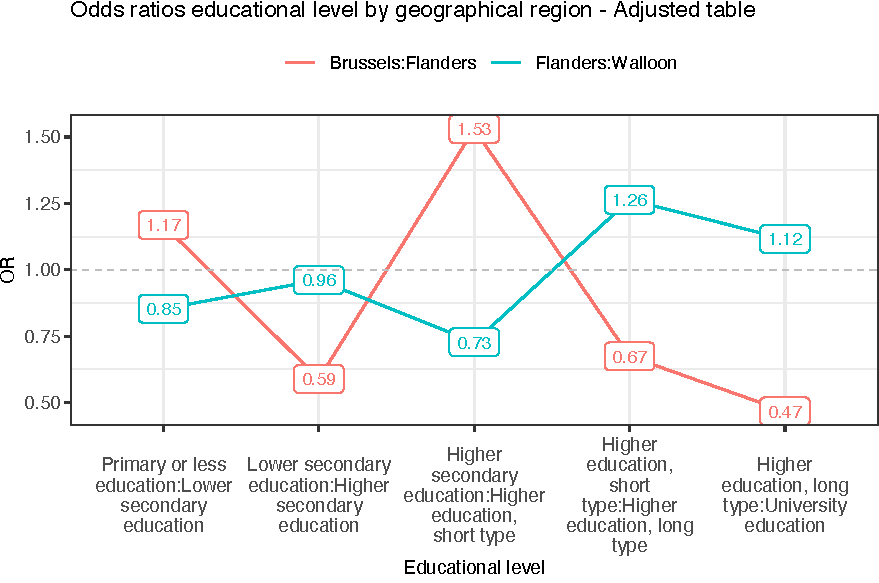
\includegraphics{Figs/tb2-1.pdf}
\caption{\label{fig:tb2}Odds ratio of adjusted table (weigthed data)}
\end{figure}


\newpage

\hypertarget{exercise-2}{%
\section{Exercise 2}\label{exercise-2}}

\begin{enumerate}
\def\labelenumi{\arabic{enumi}.}
\tightlist
\item
  Create a 4 or 5-dimensional contingency table in which one of the variables will be treated as the dependent variable. The dependent variable, and at least one of the independent variables, should have at least three categories.
\end{enumerate}

\begin{enumerate}
\def\labelenumi{\alph{enumi}.}
\tightlist
\item
  Include the table in your assignment
\end{enumerate}

\begin{table}[H]

\caption{\label{tab:tex11}Contingency table - Belgium(Flanders)}
\centering
\begin{tabular}[t]{>{\raggedright\arraybackslash}p{2.2cm}|>{\raggedright\arraybackslash}p{2.2cm}|>{\raggedright\arraybackslash}p{2.2cm}|>{\raggedleft\arraybackslash}p{1.5cm}|>{\raggedleft\arraybackslash}p{1.5cm}|>{\raggedleft\arraybackslash}p{1.5cm}|>{\raggedleft\arraybackslash}p{1.5cm}}
\hline
\multicolumn{3}{c|}{ } & \multicolumn{4}{c}{\makecell[c]{In my country immigrants are more exposed \\to unfair treatment than other groups (U)}} \\
\cline{4-7}
Immigration status (I) & Socio economical level (S) & Gender (G) & Strongly agree & Agree & Disagree & Strongly disagree\\
\hline
 &  & Boy & 34 & 133 & 71 & 9\\
\cline{3-7}
 & \multirow[t]{-2}{2.2cm}{\raggedright\arraybackslash Level 1 (lowest)} & Girl & 37 & 112 & 81 & 8\\
\cline{2-7}
 &  & Boy & 40 & 151 & 73 & 22\\
\cline{3-7}
 & \multirow[t]{-2}{2.2cm}{\raggedright\arraybackslash Level 2} & Girl & 19 & 125 & 79 & 11\\
\cline{2-7}
 &  & Boy & 36 & 205 & 123 & 19\\
\cline{3-7}
 & \multirow[t]{-2}{2.2cm}{\raggedright\arraybackslash Level 3} & Girl & 29 & 175 & 129 & 15\\
\cline{2-7}
 &  & Boy & 44 & 197 & 89 & 25\\
\cline{3-7}
\multirow[t]{-8}{2.2cm}{\raggedright\arraybackslash At least one parent born in country} & \multirow[t]{-2}{2.2cm}{\raggedright\arraybackslash Level 4 (highest)} & Girl & 33 & 160 & 96 & 24\\
\cline{1-7}
 &  & Boy & 8 & 26 & 8 & 2\\
\cline{3-7}
 & \multirow[t]{-2}{2.2cm}{\raggedright\arraybackslash Level 1 (lowest)} & Girl & 11 & 34 & 24 & 2\\
\cline{2-7}
 &  & Boy & 4 & 7 & 3 & 1\\
\cline{3-7}
 & \multirow[t]{-2}{2.2cm}{\raggedright\arraybackslash Level 2} & Girl & 6 & 14 & 3 & 3\\
\cline{2-7}
 &  & Boy & 3 & 6 & 8 & 1\\
\cline{3-7}
 & \multirow[t]{-2}{2.2cm}{\raggedright\arraybackslash Level 3} & Girl & 3 & 9 & 6 & 1\\
\cline{2-7}
 &  & Boy & 3 & 5 & 3 & 1\\
\cline{3-7}
\multirow[t]{-8}{2.2cm}{\raggedright\arraybackslash Students born in country but parent(s) born abroad} & \multirow[t]{-2}{2.2cm}{\raggedright\arraybackslash Level 4 (highest)} & Girl & 0 & 5 & 2 & 0\\
\cline{1-7}
 &  & Boy & 7 & 27 & 6 & 2\\
\cline{3-7}
 & \multirow[t]{-2}{2.2cm}{\raggedright\arraybackslash Level 1 (lowest)} & Girl & 6 & 23 & 13 & 3\\
\cline{2-7}
 &  & Boy & 3 & 9 & 7 & 0\\
\cline{3-7}
 & \multirow[t]{-2}{2.2cm}{\raggedright\arraybackslash Level 2} & Girl & 3 & 10 & 4 & 1\\
\cline{2-7}
 &  & Boy & 4 & 8 & 5 & 1\\
\cline{3-7}
 & \multirow[t]{-2}{2.2cm}{\raggedright\arraybackslash Level 3} & Girl & 4 & 10 & 3 & 0\\
\cline{2-7}
 &  & Boy & 3 & 2 & 6 & 0\\
\cline{3-7}
\multirow[t]{-8}{2.2cm}{\raggedright\arraybackslash Students and parent(s) born abroad} & \multirow[t]{-2}{2.2cm}{\raggedright\arraybackslash Level 4 (highest)} & Girl & 3 & 6 & 1 & 0\\
\hline
\multicolumn{7}{l}{\rule{0pt}{1em}\textit{Source: }}\\
\multicolumn{7}{l}{\rule{0pt}{1em}International Civic and Citizenship Education Study (ICCS) 2016}\\
\end{tabular}
\end{table}

\begin{enumerate}
\def\labelenumi{\alph{enumi}.}
\setcounter{enumi}{1}
\tightlist
\item
  Describe the variables selected
\end{enumerate}

\begin{itemize}
\tightlist
\item
  Immigration status (I): corresponds to the immigration status of the student according to the country of born of the parents of the student (\emph{At least one parent born in the country}, \emph{Students born in the country but the parent(s) born abroad} and \emph{Students and parent(s) born abroad} categories).\\
\item
  Socio-economical level (S): Level of socio-economical background, level 1 indicate the lower level, on the other hand, level 4 indicate the highest level (\emph{Level 1, level 2, level 3, level 4}).\\
\item
  Gender (G): corresponds to the gender of the student (\emph{Boy} and \emph{Girl} categories).\\
\item
  Unfair treatment (U): Dependent variable, perception of student regarding immigrants are more exposed to unfair treatment than other groups (\emph{Strongly agree}, \emph{Agree}, \emph{Disagree}, \emph{Strongly disagree} response options).
\end{itemize}

\begin{enumerate}
\def\labelenumi{\alph{enumi}.}
\setcounter{enumi}{2}
\tightlist
\item
  Formulate an initial set of hypotheses about the expected relationships between the variables (e.g.~by referring to earlier studies on the topic) Note: take care that there enough observations in your contingency table, but also not too many (e.g.~when taking data from a multi-country dataset, such as the European Social Survey or Eurobarometer, start by selecting the data from just one of the countries and focus your analysis on this country).
\end{enumerate}

Many studies have concluded that men and women differ in their attitudes towards immigrants, it is expected that this relationship is also related to the student's perception of unfair treatment towards immigrants. The immigrant background of a student is also expected to influence their perception about fair treatment, as they will have different perspectives regarding if they are the first generation of natives, second-generation or immigrants. Finally the socio-economical background it is also expected to be related to the perception studied, by associating high socio-economical background with high cultural and educational level.

\begin{enumerate}
\def\labelenumi{\arabic{enumi}.}
\setcounter{enumi}{1}
\tightlist
\item
  Use Aitkin's Simultaneous Testing Procedure, taking multiple testing into account, to draw conclusions about the different ``families of effects'' that may contain significant effects that will be important when describing the associations in the table.
\end{enumerate}

Using multiple testing, \(\gamma\) is controlled between 0.25 and 0.5 and \(\alpha\) is determined with a reasonable compromise between Type-I and Type-II errors.
We use the following formula to obtain Type I error, \(\alpha = 1-(1-\gamma)^{1/k}\) and calculate for each hypothesis P(reject at least one \(H_0\) wrongly with \(k\) tests): \(\gamma = 1-(1-\alpha)^k\).

\begin{table}[H]

\caption{\label{tab:tex12}Aitkin’s Simultaneous Testing Procedure, all $k+1$ and higher effects for $\gamma =  0.3 $}
\centering
\begin{tabular}[t]{>{\raggedright\arraybackslash}p{3cm}|>{\raggedright\arraybackslash}p{4.5cm}|>{\raggedright\arraybackslash}p{3cm}|>{\raggedright\arraybackslash}p{2cm}}
\hline
Hypothesis & Calculation of $\gamma$ & Comparison with output & Conclusion\\
\hline
$H_0:$ all $1^{st}$ \& higher=0 & $\gamma = 1-(1-0.0037)^{96}=0.299$ & 0.000<0.299 & Reject $H_0$\\
\hline
$H_0:$ all $2^{nd}$ \& higher=0 & $\gamma = 1-(1-0.0037)^{87}=0.276$ & 0.000<0.276 & Reject $H_0$\\
\hline
$H_0:$ all $3^{rd}$ \& higher=0 & $\gamma = 1-(1-0.0037)^{58}=0.193$ & 0.593>0.193 & Accept $H_0$\\
\hline
$H_0:$ all $4^{th}$ = 0 & $\gamma = 1-(1-0.0037)^{19}=0.068$ & 0.325>0.068 & Accept $H_0$\\
\hline
\end{tabular}
\end{table}

As indicated in table \ref{tab:tex12}, for \(\gamma < 0.3\) and \(\alpha=\) 0.0037, there is no evidence to reject hypotheses that all 3rd and 4th interactions are equal to 0. For \(\gamma >= 0.3\) it is possible to reject these hypotheses. This conclusion indicates that by allowing to have a Type I error of 0.0037 and Type II error of 0.3, it is necessary to only study the main effects and 2nd order interactions.

\begin{enumerate}
\def\labelenumi{\arabic{enumi}.}
\setcounter{enumi}{2}
\tightlist
\item
  (Re-)formulate the loglinear model into a multinomial logit model (using dummy coding for both the dependent and independent variables). Explain what is the most important difference between these two models (dependent quantity).
\end{enumerate}

Log-linear models describe the associations between two or more categorical variables in a statistical model, using this model and effect coding we obtain the odds of Agree/Disagree/Strongly disagree (vs.~Strongly agree)  \{UIGS\}. The dependent quantity is not the cell frequencies but the conditional odds \(f_{1|jkl}/f_{2|jkl}\). The saturated model is obtained by the following formula:

\(log(f_{1}/f_{2}) = (\lambda_1^U-\lambda_2^U) + (\lambda_1^I-\lambda_2^I) + (\lambda_1^S-\lambda_2^S) + (\lambda_1^G-\lambda_2^G) + (\lambda_{1}^{IS}-\lambda_{2}^{IS})+(\lambda_{1}^{UI}-\lambda_{2}^{UI})+(\lambda_{1}^{GI}-\lambda_{2}^{GI})+ (\lambda_{1}^{SG}-\lambda_{2}^{SG})+(\lambda_{1}^{US}-\lambda_{2}^{US})+ (\lambda_{1}^{UG}-\lambda_{2}^{UG})+ (\lambda_{1}^{ISG}-\lambda_{2}^{ISG})+ (\lambda_{1}^{ISU}-\lambda_{2}^{ISU})+(\lambda_{1}^{IGU}-\lambda_{2}^{IGU})+(\lambda_{1}^{SGU}-\lambda_{2}^{SGU})+(\lambda_{1}^{UISG}-\lambda_{2}^{UISG})\)

On the other hand, the saturated logit model with multiple response categories and dummy coding U\textbar GIS \{UGIS\} uses one variable as dependent, here conditional probabilities are calculated. The baseline-category logit model with predictors I, S and G can be obtained by the following formula: 

\(log(\frac{\pi_j}{\pi_1})=\beta_{0j}+\beta_{1j}I+\beta_{2j}S+\beta_{3j}G+\beta_{4j}IS+\beta_{5j}IG+\beta_{6j}SG+\beta_{7j}ISG\), with \(j=2,3,4\)

\begin{enumerate}
\def\labelenumi{\arabic{enumi}.}
\setcounter{enumi}{3}
\tightlist
\item
  Apply a backward selection procedure starting from the logit model with at least all 3-way interactions (also think about how to take into account the outcome of Aitkin's simultaneous testing). Evaluate the acceptable models in terms of \(L^{2}\) conditional testing and by using the AIC and BIC. Decide which model is the best fitting model.
\end{enumerate}

Likelihood ratio chi-square test will be used to evaluate how the model should be structured by removing effects. \(L^2=2\sum_i\sum_j\sum_k\sum_l f_{ijkl}log(f_{ijkl}/\hat f_{ijkl})\). Higher values compared to the saturated model, indicate better estimation.  

Akaike's Information Criterion (\(AIC=L^2-2df\)) which penalises for complexity and Bayesian Information Criterion (\(BIC=L^2-(lnN)df\)) that penalises for complexity and the number of observations is considered too. Lower negatives values are expected for the best model.  

\begin{table}[H]

\caption{\label{tab:condit}Conditional testing}
\centering
\begin{tabular}[t]{l|r|r|r|r|r|r|r|r}
\hline
Model & $L^2$ & df & p & $\Delta L^2$ & $\Delta df$ & $\Delta p$ & AIC & BIC\\
\hline
U|ISG \{ISU IGU SGU\} & 21.22 & 18 & 0.27 & 21.22 & 18 & 0.27 & -14.78 & -121.63\\
\hline
U|ISG \{ISU SGU\} & 23.97 & 24 & 0.46 & 2.75 & 6 & 0.84 & -24.03 & -166.50\\
\hline
U|ISG \{ISU GU\} & 29.67 & 33 & 0.63 & 5.70 & 9 & 0.77 & -36.33 & -232.22\\
\hline
\textbf{U|ISG \{IU SU GU\}} & \textbf{49.88} & \textbf{51} & \textbf{0.52} & \textbf{20.21} & \textbf{18} & \textbf{0.32} & \textbf{-52.12} & \textbf{-354.86}\\
\hline
\end{tabular}
\end{table}

Looking at the conditional testing for the logit model \(U|ISG\) in table \ref{tab:condit} and considering the Aitkin's simultaneous testing result, that all 3rd and higher interactions were not significantly different to zero, eliminating conditional estimations does not affect the model significantly (all p-values are greater than 0.05). This means that keeping just the 2-way interaction, which are all significant at 5\%, it is enough to have a good model. As all models have a similar fit but the last one is the less complex (more parsimonious), the homogeneous association model (no interaction term) is choose.

\begin{enumerate}
\def\labelenumi{\arabic{enumi}.}
\setcounter{enumi}{4}
\tightlist
\item
  Discuss the model fit of this best fitting model also in terms of the dissimilarity index score, pseudo R² and size of the standardized residuals.
\end{enumerate}

\begin{itemize}
\item
  By definition, Dissimilarity index takes values between 0 and 1, smaller values represent a better fit. It represents the proportion of sample cases that must move to different cells for the model to achieve a perfect fit. \(D=\sum|n_i-\hat\mu_i|/2n=\sum|p_i-\hat\pi_i|/2\).
  In the selected model, the Dissimilarity index is 0.0293 which is very close to zero, this means that a 3\% of the cases should be moved to different cells for the model to achieve a perfect fit. This percentage seems reasonable to accept it as a good fit.
\item
  Pseudo R-squared are based on explained variance between total variance(y) and error variance(e). \(R^2=\frac{S_y^2-S_e^2}{S_y^2}\)
  For this model, the pseudo R-squared measures are shown in table \ref{tab:pseudo}. It is expected that these values for logit models are between 0.1 and 0.2 to be considered a good fit. In this case, values are much lower than expected.
\end{itemize}

\begin{longtable}[]{@{}llll@{}}
\caption{\label{tab:pseudo}Pseudo R-squared measures}\tabularnewline
\toprule
& baseline & fitted & R-squared\tabularnewline
\midrule
\endfirsthead
\toprule
& baseline & fitted & R-squared\tabularnewline
\midrule
\endhead
entropy & 1.1159 & 1.1080 & 0.0071\tabularnewline
qualitative variance & 0.3094 & 0.3079 & 0.0048\tabularnewline
classification error & 0.4782 & 0.4782 & -0.0000\tabularnewline
-2/N*log-likelihood & 2.2319 & 2.2159 & 0.0071/0.0157\tabularnewline
likelihood\^{}(-2/N) & 9.3171 & 9.1698 & 0.0158/0.0177\tabularnewline
\bottomrule
\end{longtable}

\begin{itemize}
\tightlist
\item
  Standardized residuals are used to evaluate the difference between the observed frequencies and the expected frequencies, it is expected residuals to be even across the table, the largest residuals indicate where the model is least appropriate. \(res.std=\frac{n_{ij}-\hat\mu_{ij}}{\sqrt{\hat\mu_{ij}(1-p_{i+})(1-p_{+j})}}\). From all 96 residuals which their absolute value is greater than 1 are shown in table \ref{tab:res}, where -1.63 and 2.49 are the extreme values. These residuals are not considered bad, as the difference between the observed and estimated values in only one case is greater than \(\pm1.96\).
\end{itemize}

\begin{longtable}[]{@{}llll@{}}
\caption{\label{tab:res}Highest Standardized residuals in absolute values}\tabularnewline
\toprule
I S G U & observed & estimated & std. res.\tabularnewline
\midrule
\endfirsthead
\toprule
I S G U & observed & estimated & std. res.\tabularnewline
\midrule
\endhead
3 4 1 2 & 2 & 5.972 & -1.625\tabularnewline
2 2 2 3 & 3 & 7.041 & -1.523\tabularnewline
1 2 2 1 & 19 & 25.268 & -1.247\tabularnewline
3 1 1 3 & 6 & 9.423 & -1.115\tabularnewline
2 3 1 2 & 6 & 9.278 & -1.076\tabularnewline
2 4 2 1 & 0 & 1.152 & -1.073\tabularnewline
3 2 1 4 & 0 & 1.007 & -1.003\tabularnewline
3 4 2 1 & 3 & 1.691 & 1.007\tabularnewline
3 3 2 1 & 4 & 2.314 & 1.109\tabularnewline
2 3 1 3 & 8 & 4.958 & 1.366\tabularnewline
3 2 1 3 & 7 & 4.023 & 1.485\tabularnewline
3 1 2 4 & 3 & 1.298 & 1.494\tabularnewline
1 1 2 1 & 37 & 28.659 & 1.558\tabularnewline
3 4 1 3 & 6 & 2.26 & 2.488\tabularnewline
\bottomrule
\end{longtable}

\begin{enumerate}
\def\labelenumi{\arabic{enumi}.}
\setcounter{enumi}{5}
\tightlist
\item
  Your dependent variable has at least three categories (and you have used dummy coding for the dependent variable). Decide whether you will present the results and interpretation in terms of Baseline-Category Logits or Adjacent-Categories Logits. Explain your decision.
\end{enumerate}

The dependent variable, \emph{Unfair treatment (U): Perception of the student regarding immigrants are more exposed to unfair treatment than other groups} has 4 response categories. This categories are \emph{Strongly agree}, \emph{Agree}, \emph{Disagree}, \emph{Strongly disagree}, usually called Likert scale. This scale is commonly used as a nominal variable but there is an underline ordering in the categories, as the Strongly agree category corresponds to the highest presence of the studied attribute, and Strongly disagree to the lower presence of the attribute.

Considering the ordinal characteristic of the dependent variable, Adjacent-Categories Logits seem to be the best approach to interpret the results, in order to consider the entire scale. The adjacent-categories logits are calculated as \(log(\frac{\pi_{j+1}}{\pi_j})=\beta_{0j}+\beta_{1j}G+\beta_{2j}I+\beta_{3j}S\) with \(j=1,2,3\).

\begin{enumerate}
\def\labelenumi{\arabic{enumi}.}
\setcounter{enumi}{6}
\tightlist
\item
  Present the Baseline-Category or Adjacent-Categories Logits and discuss the parameter estimates, also discuss the associated odds ratios. Note: interpret at least one interaction effect. You should present your results as if you are writing a basic scientific paper; the interpretation of your results should also include a discussion on how your results fit in with the hypotheses you formulated.
\end{enumerate}

\begin{longtable}[t]{>{\raggedright\arraybackslash}p{4cm}|>{\raggedleft\arraybackslash}p{1cm}|>{\raggedleft\arraybackslash}p{1cm}|>{\raggedright\arraybackslash}p{0.6cm}|>{\raggedleft\arraybackslash}p{1cm}|>{\raggedleft\arraybackslash}p{1cm}|>{\raggedright\arraybackslash}p{0.6cm}|>{\raggedleft\arraybackslash}p{1cm}|>{\raggedleft\arraybackslash}p{1cm}|>{\raggedright\arraybackslash}p{0.6cm}}
\caption{\label{tab:models}Multinomial odds model}\\
\hline
\multicolumn{1}{c|}{ } & \multicolumn{3}{c|}{Agree} & \multicolumn{3}{c|}{Disagree} & \multicolumn{3}{c}{Strongly disagree} \\
\cline{2-4} \cline{5-7} \cline{8-10}
Coefficients & $\pi_2$ & pval &  & $\pi_3$ & pval &  & $\pi_4$ & pval & \\
\hline
(Intercept) & 3.79 & 0.0000 & *** & 2.02 & 0.0000 & *** & 0.29 & 0.0000 & ***\\
\hline
GENDER Girl & 1.11 & 0.3943 &  & 1.39 & 0.0117 & * & 1.05 & 0.8228 & \\
\hline
IMMIG Students born in country but parent(s) born abroad & 0.64 & 0.0294 & * & 0.56 & 0.0122 & * & 0.73 & 0.3915 & \\
\hline
IMMIG Students and parent(s) born abroad & 0.66 & 0.0517 &  & 0.52 & 0.0077 & ** & 0.52 & 0.1284 & \\
\hline
NISB Level 2 & 1.14 & 0.4654 &  & 1.05 & 0.8077 &  & 1.86 & 0.0395 & *\\
\hline
NISB Level 3 & 1.38 & 0.0593 &  & 1.57 & 0.0133 & * & 1.68 & 0.0860 & \\
\hline
NISB Level 4 (highest) & 1.13 & 0.4679 &  & 1.01 & 0.9458 &  & 2.05 & 0.0139 & *\\
\hline
\end{longtable}

\begin{longtable}[t]{>{\raggedright\arraybackslash}p{4cm}|>{\raggedleft\arraybackslash}p{2.5cm}|>{\raggedleft\arraybackslash}p{2.5cm}|>{\raggedleft\arraybackslash}p{3cm}}
\caption{\label{tab:models}Adjacent-Categories logits multinomial model}\\
\hline
Coefficients & \makecell[c]{$\pi_{Agree}:$\\ $\pi_{Strongly Agree}$} & \makecell[c]{$\pi_{Disagree}:$\\ $\pi_{Agree}$} & \makecell[c]{$\pi_{Strongly disagree}:$\\ $\pi_{Disagree}$}\\
\hline
(Intercept) & 3.79 & 0.53 & 0.14\\
\hline
GENDER Girl & 1.11 & 1.25 & 0.76\\
\hline
IMMIG Students born in country but parent(s) born abroad & 0.64 & 0.88 & 1.30\\
\hline
IMMIG Students and parent(s) born abroad & 0.66 & 0.79 & 1.00\\
\hline
NISB Level 2 & 1.14 & 0.92 & 1.77\\
\hline
NISB Level 3 & 1.38 & 1.14 & 1.07\\
\hline
NISB Level 4 (highest) & 1.13 & 0.89 & 2.03\\
\hline
\end{longtable}

The estimated odds of response ``Agree'' versus ``Strongly Agree'' to the scale ``In my country, immigrants are more exposed to unfair treatment than other groups'' are equal to 3.79. For girls, the estimated odds are 1.11 times those for boys, controlling for immigration status and socio-economical background. For students At least one parent born in the country, the estimated odds are 1.56/1.52 times those students born in the country but parents born abroad and those Students and parent(s) born abroad respectively controlling by gender and socio-economical background. For students in the Level 2 or level 4 in the socio-economic index, the odds of response are 1.14-1.13 times those from level 1 and 1.38 times for students in level 3 compared to students in level 1 controlling by gender and immigration status.

The estimated odds of response ``Disagree'' versus ``Agree'' are equal to 0.53 (1.89 Agree versus Disagree). For Girls, the estimated odds of response are 1.25 times those for boys, controlling for immigration status and socio-economical level. For students At least one parent born in the country, the estimated odds are 1.14/1.27 times those students born in the country but parents born abroad and those Students and parent(s) born abroad respectively controlling by gender and socio-economical background. For students with socio-economical level 3 the odds of response ``Disagree'' versus ``Agree'' are 1.14 times those students with socio-economical level 1 and 1.09/1.12 times for students from level 1 compared to level 2 and 4 respectively, controlling by gender and immigration status.

In the case of the odd of response ``Strongly disagree'' versus ``Disagree'' are equal to 0.14 (7.14 Disagree versus Strongly disagree). In this case 1.32 times higher for boys than girls. For students born in the country but parents born abroad is 1.3 times than for students with At least one parent born in the country, there is no difference in the odds for students that they and their parents born abroad compared to students with at least one parent born in the country, controlling by gender and socio-economical background. Student's in level 2 and in level 4 in the socio-economical index are 1.77/2.03 times respectively more likely to choose the response option Strongly disagree than Disagree compared to students from level 1. Students from level 3 are just 1.07 time more likely, controlling by gender and immigration status.

In summary, it is more likely a student will choose the response option ``Agree'' or ``Disagree'' than the options ``Strongly agree'' or ``Strongly disagree'' respectively. Girls are more likely to disagree with this scale and boys are more likely to agree. Students with At least one parent born in the country (ref) are more likely to disagree to this scale and on the contrary, students that parents or themselves born abroad are likely to agree. Finally, students from the higher socio-economical background are more likely to either Agree or Strongly disagree than Strongly agree compared to those at the lowest level.

\begin{longtable}[t]{>{\raggedright\arraybackslash}p{4cm}|>{\raggedleft\arraybackslash}p{2cm}|>{\raggedleft\arraybackslash}p{2cm}|>{\raggedleft\arraybackslash}p{2cm}|>{\raggedleft\arraybackslash}p{2cm}}
\caption{\label{tab:agree}Three-way interaction odds response category Agree/Strongly disagree}\\
\hline
\multicolumn{1}{c|}{ } & \multicolumn{2}{c|}{\makecell[c]{Main and interaction \\odds ratios}} & \multicolumn{2}{c}{\makecell[c]{Odds ratios with respect \\to ref category}} \\
\cline{2-3} \cline{4-5}
Immigration status & Boy & Girl & Boy & Girl\\
\hline
 & 1.000 & 1.000 &  & \\
\cline{2-3}
 & 1.000 & 1.090 &  & \\
\cline{2-3}\nopagebreak
\multirow{-3}{4cm}{\raggedright\arraybackslash At least one parent born in country} & 1.000 & 1.000 & \multirow{-3}{2cm}{\raggedleft\arraybackslash 1.000} & 
\multirow{-3}{2cm}{\raggedleft\arraybackslash 1.090} \\
\cline{1-5}\pagebreak[0]
 & 0.581 & 0.581 &  & \\
\cline{2-3}\nopagebreak
 & 1.000 & 1.090 &  & \\
\cline{2-3}\nopagebreak
\multirow{-3}{4cm}{\raggedright\arraybackslash Students born in country but parent(s) born abroad} & 1.000 & 1.186 & \multirow{-3}{2cm}{\raggedleft\arraybackslash 0.581} & \multirow{-3}{2cm}{\raggedleft\arraybackslash 0.751}\\
\cline{1-5}\pagebreak[0]
 & 0.641 & 0.641 &  & \\
\cline{2-3}\nopagebreak
 & 1.000 & 1.090 &  & \\
\cline{2-3}\nopagebreak
\multirow{-3}{4cm}{\raggedright\arraybackslash Students and parent(s) born abroad} & 1.000 & 1.045 & \multirow{-3}{2cm}{\raggedleft\arraybackslash 0.641} & \multirow{-3}{2cm}{\raggedleft\arraybackslash 0.730}\\
\hline
\end{longtable}
\newpage
\begin{longtable}[t]{>{\raggedright\arraybackslash}p{4cm}|>{\raggedleft\arraybackslash}p{2cm}|>{\raggedleft\arraybackslash}p{2cm}|>{\raggedleft\arraybackslash}p{2cm}|>{\raggedleft\arraybackslash}p{2cm}}
\caption{\label{tab:disagree}Three-way interaction odds response category Disagree/Agree}\\
\hline
\multicolumn{1}{c|}{ } & \multicolumn{2}{c|}{\makecell[c]{Main and interaction \\odds ratios}} & \multicolumn{2}{c}{\makecell[c]{Odds ratios with respect \\to ref category}} \\
\cline{2-3} \cline{4-5}
Immigration status & Boy & Girl & Boy & Girl\\
\hline
 & 1.000 & 1.000 &  & \\
\cline{2-3}
 & 1.000 & 1.411 &  & \\
\cline{2-3}\nopagebreak
\multirow{-3}{4cm}{\raggedright\arraybackslash At least one parent born in country} & 1.000 & 1.000 & \multirow{-3}{2cm}{\raggedleft\arraybackslash 1.000} & \multirow{-3}{2cm}{\raggedleft\arraybackslash 1.411}\\
\cline{1-5}\pagebreak[0]
 & 0.555 & 0.555 &  & \\
\cline{2-3}\nopagebreak
 & 1.000 & 1.411 &  & \\
\cline{2-3}\nopagebreak
\multirow{-3}{4cm}{\raggedright\arraybackslash Students born in country but parent(s) born abroad} & 1.000 & 1.036 & \multirow{-3}{2cm}{\raggedleft\arraybackslash 0.555} & \multirow{-3}{2cm}{\raggedleft\arraybackslash 0.812}\\
\cline{1-5}\pagebreak[0]
 & 0.641 & 0.641 &  & \\
\cline{2-3}\nopagebreak
 & 1.000 & 1.411 &  & \\
\cline{2-3}\nopagebreak
\multirow{-3}{4cm}{\raggedright\arraybackslash Students and parent(s) born abroad} & 1.000 & 0.662 & \multirow{-3}{2cm}{\raggedleft\arraybackslash 0.641} & \multirow{-3}{2cm}{\raggedleft\arraybackslash 0.599}\\
\hline
\end{longtable}

\begin{longtable}[t]{>{\raggedright\arraybackslash}p{4cm}|>{\raggedleft\arraybackslash}p{2cm}|>{\raggedleft\arraybackslash}p{2cm}|>{\raggedleft\arraybackslash}p{2cm}|>{\raggedleft\arraybackslash}p{2cm}}
\caption{\label{tab:stragree}Three-way interaction odds response category Strongly Disagree/Disagree}\\
\hline
\multicolumn{1}{c|}{ } & \multicolumn{2}{c|}{\makecell[c]{Main and interaction \\odds ratios}} & \multicolumn{2}{c}{\makecell[c]{Odds ratios with respect \\to ref category}} \\
\cline{2-3} \cline{4-5}
Immigration status & Boy & Girl & Boy & Girl\\
\hline
 & 1.000 & 1.000 &  & \\
\cline{2-3}
 & 1.000 & 1.019 &  & \\
\cline{2-3}\nopagebreak
\multirow{-3}{4cm}{\raggedright\arraybackslash At least one parent born in country} & 1.000 & 1.000 & \multirow{-3}{2cm}{\raggedleft\arraybackslash 1.000} & \multirow{-3}{2cm}{\raggedleft\arraybackslash 1.019}\\
\cline{1-5}\pagebreak[0]
 & 0.687 & 0.687 &  & \\
\cline{2-3}\nopagebreak
 & 1.000 & 1.019 &  & \\
\cline{2-3}\nopagebreak
\multirow{-3}{4cm}{\raggedright\arraybackslash Students born in country but parent(s) born abroad} & 1.000 & 1.122 & \multirow{-3}{2cm}{\raggedleft\arraybackslash 0.687} & \multirow{-3}{2cm}{\raggedleft\arraybackslash 0.786}\\
\cline{1-5}\pagebreak[0]
 & 0.429 & 0.429 &  & \\
\cline{2-3}\nopagebreak
 & 1.000 & 1.019 &  & \\
\cline{2-3}\nopagebreak
\multirow{-3}{4cm}{\raggedright\arraybackslash Students and parent(s) born abroad} & 1.000 & 1.422 & \multirow{-3}{2cm}{\raggedleft\arraybackslash 0.429} & \multirow{-3}{2cm}{\raggedleft\arraybackslash 0.621}\\
\hline
\end{longtable}

If the interaction effect between Immigration background and Gender with the response variable was incorporated in the model, even though the interaction is not significantly different from zero, still interpretation is possible. In tables \ref{tab:agree},\ref{tab:disagree} and \ref{tab:stragree} the odds ratios with respect to the reference categories are shown. In the first table, it is possible to indicate that the odds to agree (versus strongly agree) to the unfair treatment of immigrants for a male student born in the country but parents born abroad is about half those male students born in the country. In the second table is shown that the odds to disagree (versus agree) for a female student with at least one parent born in the country is 1.41 times male students with at least one parent born in the country. In the third table, the odds of Strongly disagree (versus disagree) for a male student that he/she and their parents born abroad is more than half those male students that at least one parent born in the country.

\newpage

\hypertarget{exercise-3}{%
\section{Exercise 3}\label{exercise-3}}

\begin{enumerate}
\def\labelenumi{\arabic{enumi}.}
\tightlist
\item
  Create a 4 or 5-dimensional table in which each variable is theoretically a measure of the same underlying latent concept. Each variable is allowed to be dichotomous.
\end{enumerate}

Table \ref{tab:ex3} indicates the 5 items that will be used from the International Civic and Citizenship Education Study 2016, these items underlying one latent concept called \emph{Attitudes towards immigrants}. The original variables included 4 response categories (Strongly agree, Agree, Disagree and Strongly disagree), for this exercise the variables were recoded into two responses categories (Agree and Disagree). The item wording is as follows: \\
- Immigrant children should have the same opportunities for education (E).\\
- Immigrants who live in a country for several years should have the opportunity to vote (V).\\
- Immigrants should have the opportunity to continue their own customs and lifestyle (C).\\
- Immigrants should have the same rights that everyone else in the country has (R).\\
- Immigrants should have the opportunity to continue speaking their own language (L).

\begin{table}[H]

\caption{\label{tab:ex3}Contingency table - Belgium(Flanders)}
\centering
\begin{tabular}[t]{>{\raggedright\arraybackslash}p{2.5cm}|>{\raggedright\arraybackslash}p{2.5cm}|>{\raggedright\arraybackslash}p{2.5cm}|>{\raggedright\arraybackslash}p{2.5cm}|>{\raggedleft\arraybackslash}p{2cm}|>{\raggedleft\arraybackslash}p{2cm}}
\hline
\multicolumn{4}{c|}{ } & \multicolumn{2}{c}{\makecell[c]{Speak their own \\language (L)}} \\
\cline{5-6}
Opportunities for education (E) & Opportunity to vote (V) & Customs and lifestyle (C) & Same rights (R) & Agree & Disagree\\
\hline
 &  &  & Agree & 1134 & 355\\
\cline{4-6}
 &  & \multirow[t]{-2}{2.5cm}{\raggedright\arraybackslash Agree} & Disagree & 30 & 24\\
\cline{3-6}
 &  &  & Agree & 174 & 333\\
\cline{4-6}
 & \multirow[t]{-4}{2.5cm}{\raggedright\arraybackslash Agree} & \multirow[t]{-2}{2.5cm}{\raggedright\arraybackslash Disagree} & Disagree & 11 & 47\\
\cline{2-6}
 &  &  & Agree & 125 & 89\\
\cline{4-6}
 &  & \multirow[t]{-2}{2.5cm}{\raggedright\arraybackslash Agree} & Disagree & 25 & 25\\
\cline{3-6}
 &  &  & Agree & 52 & 181\\
\cline{4-6}
\multirow[t]{-8}{2.5cm}{\raggedright\arraybackslash Agree} & \multirow[t]{-4}{2.5cm}{\raggedright\arraybackslash Disagree} & \multirow[t]{-2}{2.5cm}{\raggedright\arraybackslash Disagree} & Disagree & 16 & 72\\
\cline{1-6}
 &  &  & Agree & 19 & 11\\
\cline{4-6}
 &  & \multirow[t]{-2}{2.5cm}{\raggedright\arraybackslash Agree} & Disagree & 1 & 4\\
\cline{3-6}
 &  &  & Agree & 6 & 10\\
\cline{4-6}
 & \multirow[t]{-4}{2.5cm}{\raggedright\arraybackslash Agree} & \multirow[t]{-2}{2.5cm}{\raggedright\arraybackslash Disagree} & Disagree & 7 & 7\\
\cline{2-6}
 &  &  & Agree & 4 & 3\\
\cline{4-6}
 &  & \multirow[t]{-2}{2.5cm}{\raggedright\arraybackslash Agree} & Disagree & 3 & 6\\
\cline{3-6}
 &  &  & Agree & 4 & 18\\
\cline{4-6}
\multirow[t]{-8}{2.5cm}{\raggedright\arraybackslash Disagree} & \multirow[t]{-4}{2.5cm}{\raggedright\arraybackslash Disagree} & \multirow[t]{-2}{2.5cm}{\raggedright\arraybackslash Disagree} & Disagree & 6 & 48\\
\hline
\multicolumn{6}{l}{\rule{0pt}{1em}\textit{Source: }}\\
\multicolumn{6}{l}{\rule{0pt}{1em}International Civic and Citizenship Education Study (ICCS) 2016}\\
\end{tabular}
\end{table}

\begin{enumerate}
\def\labelenumi{\arabic{enumi}.}
\setcounter{enumi}{1}
\tightlist
\item
  Test whether the items actually measure one latent variable by performing an exploratory latent class analysis, paying attention to the number of latent classes. Discuss each step in terms of model fit and draw your conclusion about the final model.
\end{enumerate}

In table \ref{tab:lca1} summarizes the exploratory latent class analysis, non-independence model (null model/1 class) is not enough to explain the amount of association in the data, therefore more than 1 class is needed. The second model, with 2 classes reduces the L2 in 86\% but still not acceptable with 20 degrees of freedom. If another class is added to the model, an 81\% is reduced and 97\% compared to the baseline model, but this model it does not have an adequate fit accordingly to \(L2\) test. Finally, if a 4th class is added the model, this does is not identified, 2 boundary estimates are found, i.e., the model does not reach a global maxima as the results are different by using different starting values. For this, one of the solutions is to add a restriction and check for stability of the results by changing the starting values.

\begin{table}[H]

\caption{\label{tab:lca1}Model fit for different number of classes}
\centering
\begin{tabu} to \linewidth {>{\raggedright}X>{\raggedleft}X>{\raggedleft}X>{\raggedleft}X>{\raggedleft}X>{\raggedleft}X>{\raggedleft}X>{\raggedleft}X}
\hline
Classes & $\chi^2$ & $L^2$ & df & p-value & $\Delta L^2$ & AIC & BIC\\
\hline
1 & 4686.6 & 1363.5 & 26 & 0.000 &  & 13984.3 & 14014.0\\
\hline
2 & 255.7 & 195.3 & 20 & 0.000 & -1168 & 12828.0 & 12893.5\\
\hline
3 & 42.6 & 36.8 & 14 & 0.001 & -158 & 12681.6 & 12782.8\\
\hline
4 & 14.8 & 13.0 & 8 & 0.111 & -24 & 12669.8 & 12806.7\\
\hline
\textbf{$4^{a}$} & \textbf{14.8} & \textbf{13.1} & \textbf{9} & \textbf{0.156} & \textbf{0} & \textbf{12798.9} & \textbf{12667.9}\\
\hline
\multicolumn{8}{l}{\rule{0pt}{1em}\textit{Note: }}\\
\multicolumn{8}{l}{\rule{0pt}{1em}a: Exact indicator imposed}\\
\end{tabu}
\end{table}

\begin{enumerate}
\def\labelenumi{\arabic{enumi}.}
\setcounter{enumi}{2}
\tightlist
\item
  Discuss the results of your final latent class model in terms of the size and characteristics of the latent classes identified in your analysis.
\end{enumerate}

In the four-class model, 2 boundary estimates were found concerning variables ``Same rights (R)'' and ``Customs and lifestyle (C)''. In order to obtain a reliable model with 4 classes, the probability of variable R in class 1 was fixed to 1, as the estimated value is close to this value even in previous models.\\
Using this fixation it is possible to obtain goodness of fit acceptable, is worth to mention that stability of the model is maintained after changing the starting values, probabilities and class size estimations only vary at the 3rd decimal.

In table \ref{tab:cond1} it possible to see that the size classes for three classes are 60\% for High Engagement students, 31\% for the Medium Engagement students and 9\% for No Engagement students. In table \ref{tab:cond2} the additional class estimated reduce the first class of High Engagement students to 54\%, but maintain Medium Engagement students class in 31\%. The No Engagement class is reduced to 8\% and the Basic Engagement students class appears with a sample size of 7\%. A degree of freedom is gain by the constrain.

In summary, students can be classified correctly in 3 groups but more specific into 4 and with a goodness of fit adequate, where the group of Basic Engagement differentiate the students that consider that immigrants can continue with their customs and lifestyle and receive the same opportunities for education, but they are less likely to agree with their opportunity to keep speaking their language, to have the same rights and to vote. A clear description can be visualized in figure \ref{fig:cond2}.

\begin{table}[H]

\caption{\label{tab:cond1}Conditional probabilities (three latent classes)}
\centering
\begin{tabular}[t]{>{\raggedright\arraybackslash}p{3.5cm}|>{\raggedright\arraybackslash}p{2cm}|>{\raggedleft\arraybackslash}p{2.5cm}|>{\raggedleft\arraybackslash}p{2.5cm}|>{\raggedleft\arraybackslash}p{2.5cm}}
\hline
Items & Responses & High Engagement & Medium Engagement & No Engagement\\
\hline
 & Agree & \textcolor{cyan}{\textbf{0.912}} & \textcolor{black}{0.273} & \textcolor{black}{0.245}\\
\cline{2-5}
\multirow[t]{-2}{3.5cm}{\raggedright\arraybackslash Customs and lifestyle (C)} & Disagree & \textcolor{black}{0.088} & \textcolor{blue}{\textbf{0.727}} & \textcolor{red}{\textbf{0.755}}\\
\cline{1-5}
 & Agree & \textcolor{cyan}{\textbf{0.982}} & \textcolor{blue}{\textbf{0.973}} & \textcolor{red}{\textbf{0.625}}\\
\cline{2-5}
\multirow[t]{-2}{3.5cm}{\raggedright\arraybackslash Opportunities for education (E)} & Disagree & \textcolor{black}{0.018} & \textcolor{black}{0.027} & \textcolor{black}{0.375}\\
\cline{1-5}
 & Agree & \textcolor{cyan}{\textbf{0.821}} & \textcolor{black}{0.178} & \textcolor{black}{0.232}\\
\cline{2-5}
\multirow[t]{-2}{3.5cm}{\raggedright\arraybackslash Speak their own language (L)} & Disagree & \textcolor{black}{0.179} & \textcolor{blue}{\textbf{0.822}} & \textcolor{red}{\textbf{0.768}}\\
\cline{1-5}
 & Agree & \textcolor{cyan}{\textbf{0.973}} & \textcolor{blue}{\textbf{0.914}} & \textcolor{black}{0.234}\\
\cline{2-5}
\multirow[t]{-2}{3.5cm}{\raggedright\arraybackslash Same rights (R)} & Disagree & \textcolor{black}{0.027} & \textcolor{black}{0.086} & \textcolor{red}{\textbf{0.766}}\\
\cline{1-5}
 & Agree & \textcolor{cyan}{\textbf{0.906}} & \textcolor{blue}{\textbf{0.657}} & \textcolor{black}{0.212}\\
\cline{2-5}
\multirow[t]{-2}{3.5cm}{\raggedright\arraybackslash Opportunity to vote (V)} & Disagree & \textcolor{black}{0.094} & \textcolor{black}{0.343} & \textcolor{red}{\textbf{0.788}}\\
\cline{1-5}
\textbf{Latent Class Size} & \textbf{} & \textbf{\textcolor{black}{\textbf{0.598}}} & \textbf{\textcolor{black}{0.306}} & \textbf{\textcolor{black}{0.097}}\\
\hline
\multicolumn{5}{l}{\rule{0pt}{1em}\textit{$L^2$ =  36.811 , df =  15 ,p =  0.001}}\\
\multicolumn{5}{l}{\rule{0pt}{1em}$\chi^2$ =  42.637}\\
\end{tabular}
\end{table}

\begin{figure}
\centering
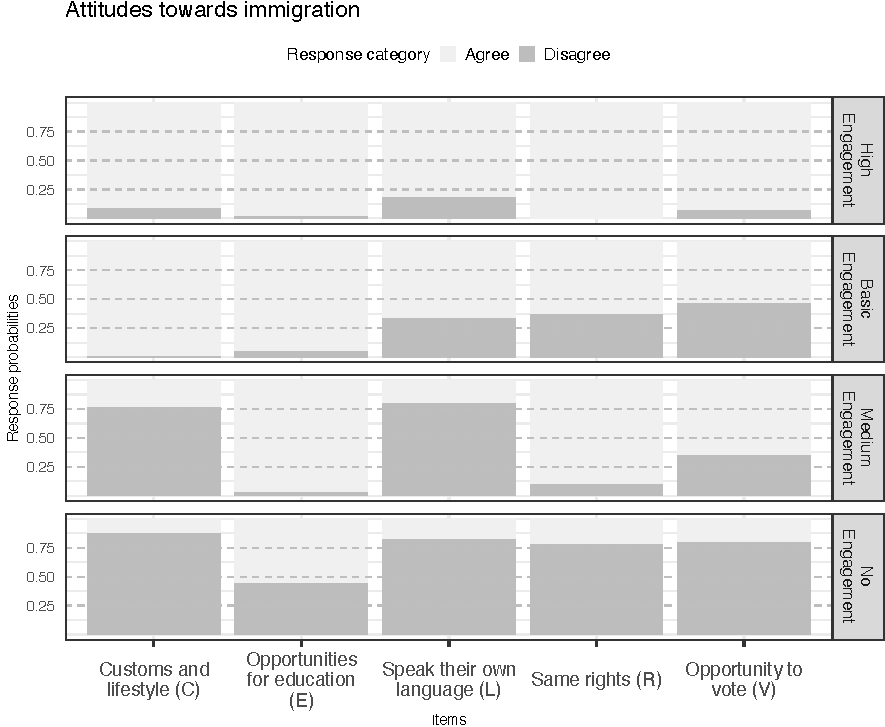
\includegraphics{Figs/cond2-1.pdf}
\caption{\label{fig:cond2}Main response probabilities by classes}
\end{figure}


\begin{table}[H]

\caption{\label{tab:cond2}Conditional probabilities (four latent classes) with exact restriction}
\centering
\begin{tabular}[t]{>{\raggedright\arraybackslash}p{3.5cm}|>{\raggedright\arraybackslash}p{2cm}|>{\raggedleft\arraybackslash}p{2.5cm}|>{\raggedleft\arraybackslash}p{2.5cm}|>{\raggedleft\arraybackslash}p{2.5cm}|>{\raggedleft\arraybackslash}p{2.5cm}}
\hline
Items & Responses & High Engagement & Basic Engagement & Medium Engagement & No Engagement\\
\hline
 & Agree & \textcolor{cyan}{\textbf{0.9176}} & \textcolor{magenta}{\textbf{0.9954}} & \textcolor{black}{0.2346} & \textcolor{black}{0.1252}\\
\cline{2-6}
\multirow[t]{-2}{3.5cm}{\raggedright\arraybackslash Customs and lifestyle (C)} & Disagree & \textcolor{black}{0.0824} & \textcolor{black}{0.0046} & \textcolor{blue}{\textbf{0.7654}} & \textcolor{red}{\textbf{0.8748}}\\
\cline{1-6}
 & Agree & \textcolor{cyan}{\textbf{0.9832}} & \textcolor{magenta}{\textbf{0.9549}} & \textcolor{blue}{\textbf{0.9729}} & \textcolor{red}{\textbf{0.5568}}\\
\cline{2-6}
\multirow[t]{-2}{3.5cm}{\raggedright\arraybackslash Opportunities for education (E)} & Disagree & \textcolor{black}{0.0168} & \textcolor{black}{0.0451} & \textcolor{black}{0.0271} & \textcolor{black}{0.4432}\\
\cline{1-6}
 & Agree & \textcolor{cyan}{\textbf{0.816}} & \textcolor{magenta}{\textbf{0.6628}} & \textcolor{black}{0.2037} & \textcolor{black}{0.1817}\\
\cline{2-6}
\multirow[t]{-2}{3.5cm}{\raggedright\arraybackslash Speak their own language (L)} & Disagree & \textcolor{black}{0.184} & \textcolor{black}{0.3372} & \textcolor{blue}{\textbf{0.7963}} & \textcolor{red}{\textbf{0.8183}}\\
\cline{1-6}
 & Agree & \textcolor{cyan}{\textbf{1.000$^a$}} & \textcolor{magenta}{\textbf{0.6309}} & \textcolor{blue}{\textbf{0.9051}} & \textcolor{black}{0.2224}\\
\cline{2-6}
\multirow[t]{-2}{3.5cm}{\raggedright\arraybackslash Same rights (R)} & Disagree & \textcolor{black}{0.000} & \textcolor{black}{0.3691} & \textcolor{black}{0.0949} & \textcolor{red}{\textbf{0.7776}}\\
\cline{1-6}
 & Agree & \textcolor{cyan}{\textbf{0.9352}} & \textcolor{magenta}{\textbf{0.5413}} & \textcolor{blue}{\textbf{0.6516}} & \textcolor{black}{0.2038}\\
\cline{2-6}
\multirow[t]{-2}{3.5cm}{\raggedright\arraybackslash Opportunity to vote (V)} & Disagree & \textcolor{black}{0.0648} & \textcolor{black}{0.4587} & \textcolor{black}{0.3484} & \textcolor{red}{\textbf{0.7962}}\\
\cline{1-6}
\textbf{Latent Class Size} & \textbf{} & \textbf{\textcolor{black}{0.5417}} & \textbf{\textcolor{black}{0.0733}} & \textbf{\textcolor{black}{0.3074}} & \textbf{\textcolor{black}{0.0775}}\\
\hline
\multicolumn{6}{l}{\rule{0pt}{1em}\textit{$L^2$ = 13.1435, df = 9, p =  0.156}}\\
\multicolumn{6}{l}{\rule{0pt}{1em}$\chi^2$ = 14.8099}\\
\multicolumn{6}{l}{\rule{0pt}{1em}\textsuperscript{a} Exact indicator imposed}\\
\end{tabular}
\end{table}

\begin{enumerate}
\def\labelenumi{\arabic{enumi}.}
\setcounter{enumi}{3}
\tightlist
\item
  Formulate at least two hypotheses for a confirmatory latent class analysis. Impose the restrictions for your hypothesis on the model, and draw conclusions.
\end{enumerate}

One of the hypothesis that is clear to see is that in High Engagement class, student's probabilities are the same as for students in Basic engagement class for variables \emph{Customs and lifestyle (C)} and \emph{Opportunities for education (E)}.

The second hypothesis to be tested is establishing that students in Medium Engagement class and students that are in No Engagement class have the same probability to disagree with the item \emph{Speak their own language (L)}.

These restrictions are imposed by adding the following code:
\begin{verbatim}
X
E|X eq2
V|X
C|X eq2
R|X eq2
L|X eq2
des [1 0 0 0 0 0 1 0
     2 5 0 0 0 0 2 5
     0 0 0 0 0 0 -1 0
     0 0 4 3 4 3 0 0 ]
sta R|X [.5 .5 .9 .1 .2 .8 1 0]
\end{verbatim}

With this restriction, the model improves its fit, $L^2$ increase to 14.18 with 3 more degrees of freedom (12). Sample sizes are adjusted to 54\%, 29\%, 8\% and 9\% respectively as indicated in table \ref{tab:conf1}.

In conclusion, the latent class analysis performed gives 4 latent classes, the first class, called ``High Engagement'' is composed by students who are likely to agree with all items analysed regarding their attitudes towards immigrants, they agree to that they should maintain their customs and lifestyle, Have equal opportunities for education, that they should speak their own language, Have the same rights and opportunity to vote. There is a second class which is differentiated from this one is that students even though they are highly likely to agree with items like immigrants should maintain their customs and lifestyle and they should have opportunities for education, they are not equally likely to agree to items regarding speak their own language, have the same rights and the opportunity to vote, this class was called as Basic engagement.\\
In the third class, called Moderate engagement, students are more likely to agree with that immigrant should have opportunity to education and same rights as any other citizen and at some level with their opportunity to vote but they are highly likely to disagree with immigrants speaking their own language and maintaining their customs and lifestyle. In the last class, called No Engagement, students are highly likely to disagree with all items but tend to agree with at least opportunity for education.

\begin{table}[H]

\caption{\label{tab:conf1}Conditional probabilities (four latent classes) with equality restrictions}
\centering
\begin{tabular}[t]{>{\raggedright\arraybackslash}p{3.5cm}|>{\raggedright\arraybackslash}p{2cm}|>{\raggedleft\arraybackslash}p{2.5cm}|>{\raggedleft\arraybackslash}p{2.5cm}|>{\raggedleft\arraybackslash}p{2.5cm}|>{\raggedleft\arraybackslash}p{2.5cm}}
\hline
Items & Responses & High Engagement & Basic Engagement & Medium Engagement & No Engagement\\
\hline
 & Agree & \textcolor{cyan}{\textbf{0.9126$^b$}} & \textcolor{magenta}{\textbf{0.9126$^b$}} & \textcolor{black}{0.2289} & \textcolor{black}{0.1476}\\
\cline{2-6}
\multirow[t]{-2}{3.5cm}{\raggedright\arraybackslash Customs and lifestyle (C)} & Disagree & \textcolor{black}{0.0874} & \textcolor{black}{0.0874} & \textcolor{blue}{\textbf{0.7711}} & \textcolor{red}{\textbf{0.8524}}\\
\cline{1-6}
 & Agree & \textcolor{cyan}{\textbf{0.9809$^b$}} & \textcolor{magenta}{\textbf{0.9809$^b$}} & \textcolor{blue}{\textbf{0.9743}} & \textcolor{red}{\textbf{0.5546}}\\
\cline{2-6}
\multirow[t]{-2}{3.5cm}{\raggedright\arraybackslash Opportunities for education (E)} & Disagree & \textcolor{black}{0.0191} & \textcolor{black}{0.0191} & \textcolor{black}{0.0257} & \textcolor{black}{0.4454}\\
\cline{1-6}
 & Agree & \textcolor{cyan}{\textbf{0.8149}} & \textcolor{magenta}{\textbf{0.6752}} & \textcolor{black}{0.1825} & \textcolor{black}{0.1825}\\
\cline{2-6}
\multirow[t]{-2}{3.5cm}{\raggedright\arraybackslash Speak their own language (L)} & Disagree & \textcolor{black}{0.1851} & \textcolor{black}{0.3248} & \textcolor{blue}{\textbf{0.8175$^b$}} & \textcolor{red}{\textbf{0.8175$^b$}}\\
\cline{1-6}
 & Agree & \textcolor{cyan}{\textbf{1.0000$^a$}} & \textcolor{magenta}{\textbf{0.6796}} & \textcolor{blue}{\textbf{0.9093}} & \textcolor{black}{0.2298}\\
\cline{2-6}
\multirow[t]{-2}{3.5cm}{\raggedright\arraybackslash Same rights (R)} & Disagree & \textcolor{black}{0.0000} & \textcolor{black}{0.3204} & \textcolor{black}{0.0907} & \textcolor{red}{\textbf{0.7702}}\\
\cline{1-6}
 & Agree & \textcolor{cyan}{\textbf{0.9393}} & \textcolor{magenta}{\textbf{0.5528}} & \textcolor{blue}{\textbf{0.6506}} & \textcolor{black}{0.2108}\\
\cline{2-6}
\multirow[t]{-2}{3.5cm}{\raggedright\arraybackslash Opportunity to vote (V)} & Disagree & \textcolor{black}{0.0607} & \textcolor{black}{0.4472} & \textcolor{black}{0.3494} & \textcolor{red}{\textbf{0.7892}}\\
\cline{1-6}
\textbf{Latent Class Size} & \textbf{} & \textbf{\textcolor{black}{0.5393}} & \textbf{\textcolor{black}{0.0889}} & \textbf{\textcolor{black}{0.2919}} & \textbf{\textcolor{black}{0.0799}}\\
\hline
\multicolumn{6}{l}{\rule{0pt}{1em}\textit{$L^2$ = 14.1792, df = 12,p =  0.289}}\\
\multicolumn{6}{l}{\rule{0pt}{1em}$\chi^2$ = 15.6664}\\
\multicolumn{6}{l}{\rule{0pt}{1em}\textsuperscript{a} Exact indicator imposed}\\
\multicolumn{6}{l}{\rule{0pt}{1em}\textsuperscript{b} Equality restriction imposed}\\
\end{tabular}
\end{table}

\end{document}
